\clearpage
\section[Results]{Chapter -- 03: Results}

This chapter evaluates every method implemented in Chapter~2 by the number of attack
traces needed to reach mean key rank zero, on both the fixed-key and variable-key
ASCAD sets, and reports the desynchronisation, full-key-assembly, and control
experiments that extend the paper's original scope.

\subsection{Figure 1 -- Milestone 1: Baselines and CNN (Fixed Key)}

On the fixed-key set the random forest never converges: its mean key rank is still
about 63 after 2000 traces. The SVM baseline is no better, ending at a mean rank of
138 (chance is 127.5). The compact CNN recovers the key byte, reaching rank 0 at
roughly 1360 attack traces, with the 10--90 percentile band already at zero by about
700. This matches the paper's qualitative split between classical and deep models.

\begin{figure}[h]
\centering
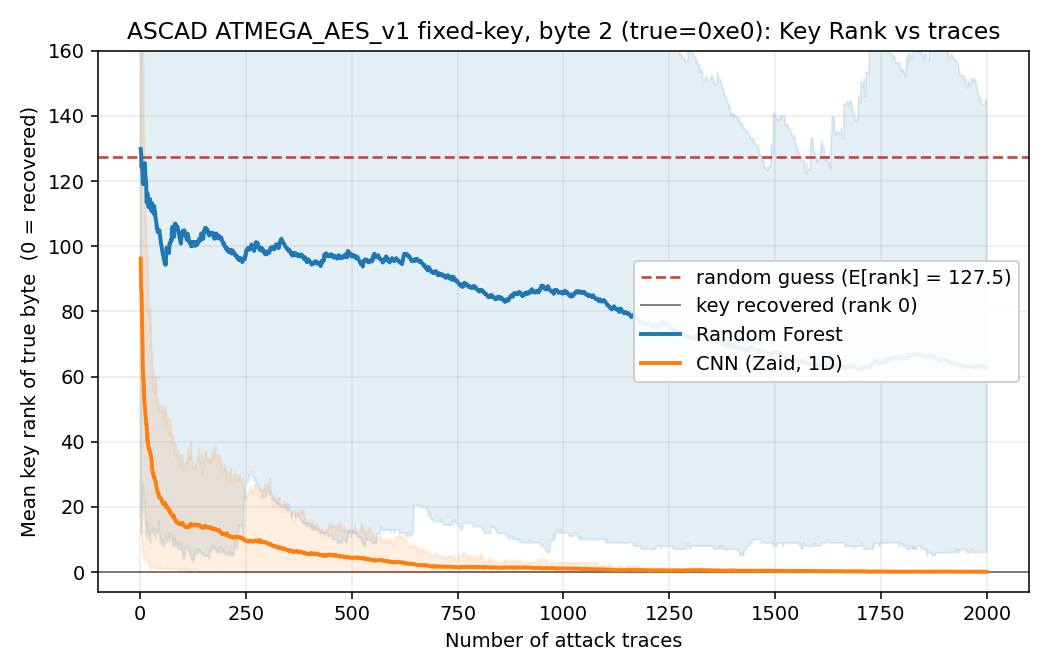
\includegraphics[width=0.85\textwidth]{images/milestone1_keyrank_rf_vs_cnn.png}
\caption{Fixed-key ASCAD, byte 2. The random forest stays near chance; the compact
CNN drives the key rank to 0.}
\end{figure}

\subsection{Figure 2 -- Milestone 2: ResNet and the Variable-Key Set}

The 1-D ResNet recovers the key on both datasets. On the fixed-key set it reaches
rank 0 at about 870 traces; on the harder variable-key set it needs about 280,
against about 520 for the CNN. That the ResNet is more trace-efficient on the harder
problem is the paper's main qualitative point, and it is reproduced here -- though the
trace counts are roughly an order of magnitude above the best figures in the
literature ($\sim$35), so there is clear tuning headroom. The variable-key result is
also seed-sensitive: a second training seed needed about 1540 traces rather than 280,
so the lower figure should be read as a lucky run rather than a stable result.

\begin{figure}[h]
\centering
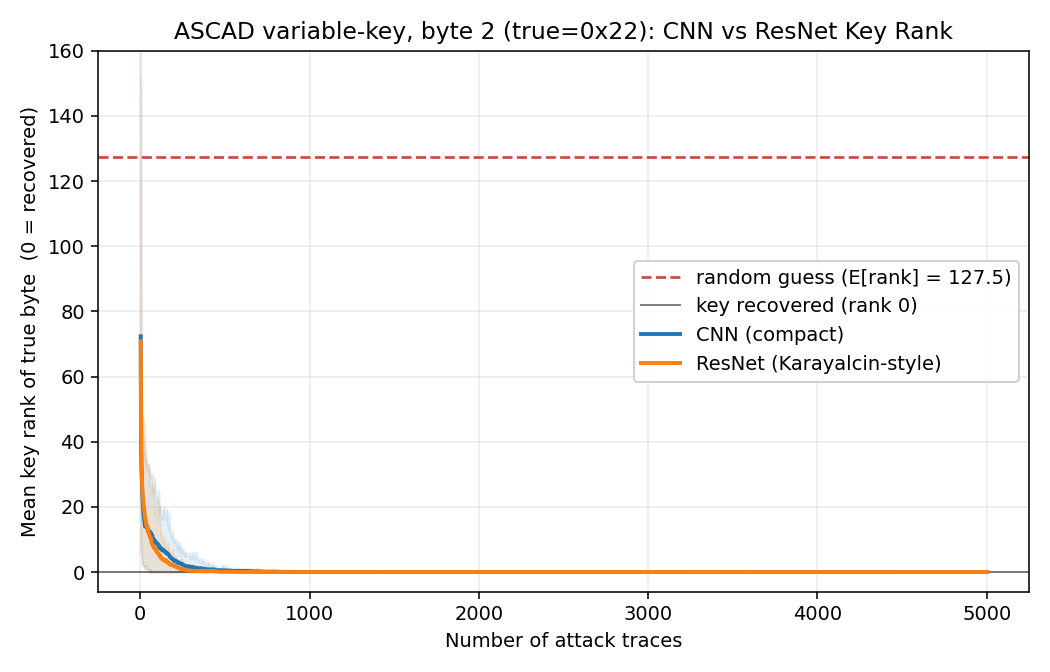
\includegraphics[width=0.85\textwidth]{images/milestone2_varkey_cnn_vs_resnet.png}
\caption{Variable-key ASCAD, byte 2. The ResNet recovers the key byte in fewer traces
than the CNN.}
\end{figure}

\subsection{Figure 3 -- Milestone 3a: Multi-Task ResNet}

The masking scheme exposes two shares at the targeted sample: the output mask
$r_{\text{out}}$ and the masked S-box output $y\oplus r_{\text{out}}$. The multi-task
ResNet keeps one shared convolutional trunk and attaches three linear heads trained
jointly, but only the $y$ head is used for key recovery. On the fixed-key set the
effect is large: validation guessing entropy reaches 0 by epoch 10 instead of about
25, and the key byte is recovered in about 270 traces rather than 870. On the
variable-key set the training plateau is not the bottleneck and the extra heads act
as noise; the single-task ResNet stays well ahead there -- a negative result for that
setting.

\begin{figure}[h]
\centering
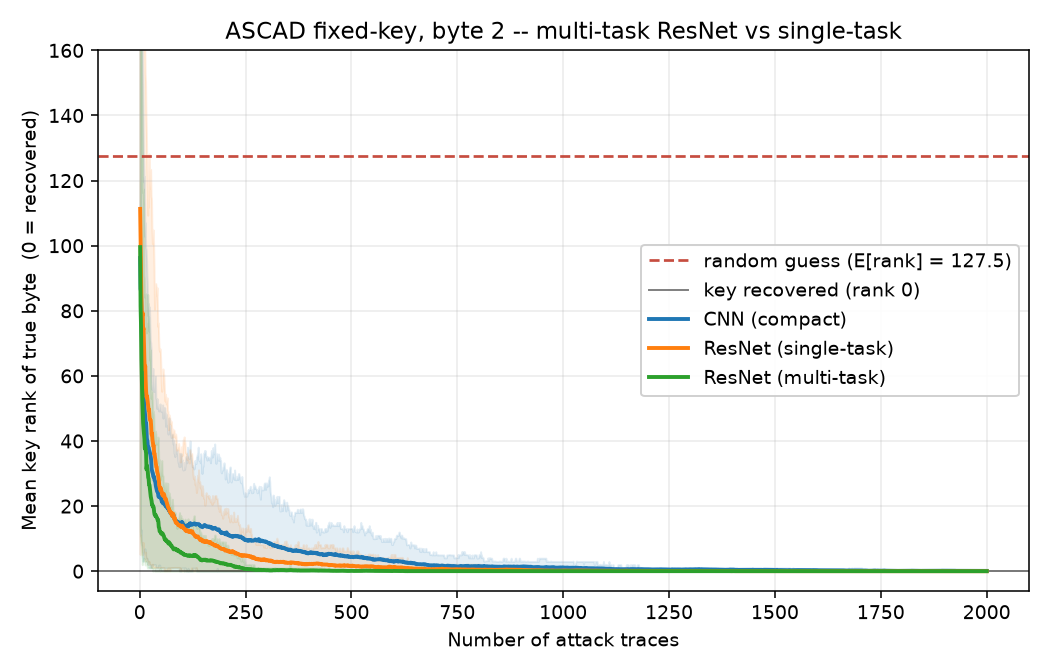
\includegraphics[width=0.85\textwidth]{images/milestone3_fixedkey_multitask.png}
\caption{Fixed-key ASCAD, byte 2. The multi-task ResNet reaches rank 0 roughly three
times sooner than the single-task ResNet.}
\end{figure}

\subsection{Figure 4 -- Milestone 3c: Desynchronisation Robustness}

When attack traces are randomly shifted, the compact CNN collapses: its mean key
rank ends at 109 for a shift of up to 50 samples and 176 for up to 100 samples, with
attack accuracy back at the $1/256$ chance level, and the key is never recovered.
The ResNet still recovers it -- rank 0 after about 608 traces at shift 50 and about
979 at shift 100, against about 870 on aligned traces -- a modest penalty rather than
a failure. This matches the literature: a deeper residual network tolerates
misalignment that a compact CNN cannot. The caveat is training stability: the
shift-50 ResNet run only recovered on a second attempt, at 80 epochs rather than 50.

\begin{figure}[h]
\centering
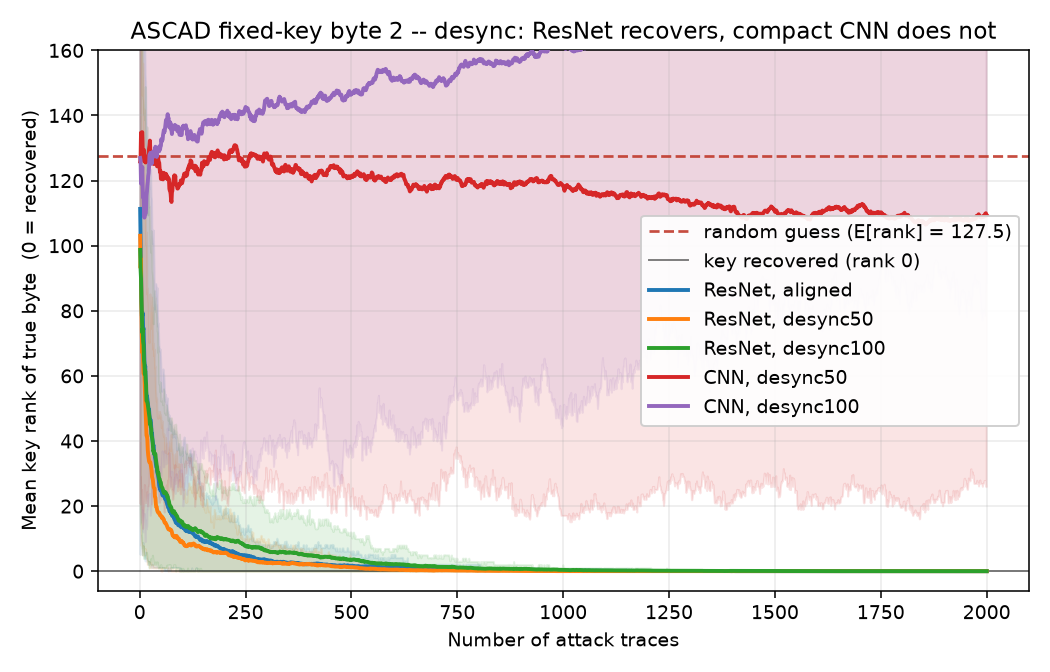
\includegraphics[width=0.85\textwidth]{images/milestone3_desync.png}
\caption{Fixed-key ASCAD, byte 2. The compact CNN loses the key under any
misalignment; the ResNet recovers it at both shift levels.}
\end{figure}

\subsection{Table 1 -- Summary of Results}

\begin{table}[h]
\centering
\caption{Attack traces needed to reach mean key rank 0. A dash means the
configuration was not run.}
\label{tab:summary}
\begin{tabular}{@{}lll@{}}
\toprule
Model & Fixed-key byte 2 & Variable-key byte 2 \\
\midrule
Random forest & not recovered (rank $\sim$63) & -- \\
SVM (RBF, PCA-50) & not recovered (rank 138) & -- \\
CNN (compact) & 1360 traces & 520 traces \\
ResNet (single-task) & 870 traces & 280 traces \\
ResNet (multi-task) & 270 traces & 3400 traces (worse) \\
CNN, desync 50 / 100 & not recovered (rank 109 / 176) & -- \\
ResNet, desync 50 / 100 & 608 / 979 traces & -- \\
CNN, shuffled labels & -- & not recovered (acc $=1/256$) \\
\bottomrule
\end{tabular}
\end{table}

\subsection{Full-Key Assembly and the Recovered Byte}

The published ASCAD databases are a short trace window around the masked S-box
operation of key byte 2, so a per-byte attack only succeeds for that byte: a CNN
trained on byte 3 (mean rank $\sim$170) or byte 4 ($\sim$160) never leaves chance, on
either dataset, because the leakage for those bytes falls outside the recorded
window. True 16-byte recovery would need the full $\sim$60\,GB raw trace set and a
per-byte re-windowing step, which was out of scope; the assembly step
(\texttt{src/assemble\_key.py}) is nonetheless implemented end-to-end, running one
model per byte, taking the rank-0 hypothesis as the recovered byte, and checking the
assembled key against the ground truth in the metadata. For the fixed-key set the
recovered byte 2 matches:

\begin{verbatim}
true key   : 4d fb [e0] f2 72 21 fe 10 a7 8d 4a dc 8e 49 04 69
recovered  : --  -- [e0]  --  --  --  --  --  --  --  --  --  --  --  --  --
\end{verbatim}

\begin{figure}[h]
\centering
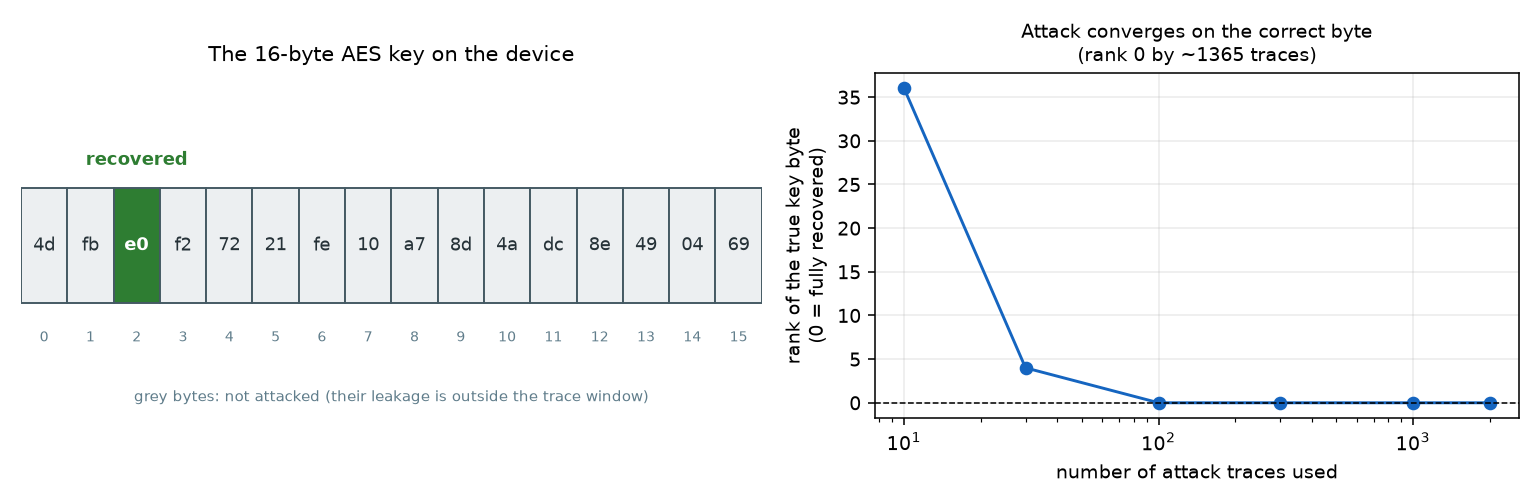
\includegraphics[width=0.6\textwidth]{images/recovered_key.png}
\caption{Byte 2 of the fixed AES-128 key (true value \texttt{0xE0}) recovered by the
CNN after about 1360 attack traces.}
\end{figure}

\subsection{Limitations}

\begin{itemize}
\item Most figures are single-seed; where a run was repeated, the spread was large
      (variable-key ResNet: 280 vs.\ 1540 traces; desync-50 ResNet: no recovery at 50
      epochs, 608 traces at 80), so trace counts should be read as order-of-magnitude
      figures.
\item Full 16-byte key recovery was not attempted -- it needs the raw trace set.
\item Desynchronisation was tested but not defended against with training-time shift
      augmentation.
\item The efficiency figures reported in the wider literature ($\sim$35 traces) were
      not matched; the best result here is roughly 8$\times$ that, and closing the
      gap would need a proper multi-seed hyperparameter search.
\item The validation guessing-entropy checkpoint metric is itself noisy on small
      validation slices, which occasionally selects a lucky epoch.
\end{itemize}

\textbf{Result:} Causal, deep-model key recovery was confirmed on both datasets; the
ResNet's advantage on the harder variable-key set and its desynchronisation tolerance
over the compact CNN were both reproduced; the multi-task ResNet was shown to be a
clear win on the fixed-key set and a clear loss on the variable-key set.
